%%%%%%%% ICML 2021 EXAMPLE LATEX SUBMISSION FILE %%%%%%%%%%%%%%%%%

\documentclass{article}

% Recommended, but optional, packages for figures and better typesetting:
\usepackage{microtype}
\usepackage{graphicx}
\usepackage{subfigure}
\usepackage{booktabs} % for professional tables

% hyperref makes hyperlinks in the resulting PDF.
% If your build breaks (sometimes temporarily if a hyperlink spans a page)
% please comment out the following usepackage line and replace
% \usepackage{icml2021} with \usepackage[nohyperref]{icml2021} above.
\usepackage{hyperref}

% Attempt to make hyperref and algorithmic work together better:
\newcommand{\theHalgorithm}{\arabic{algorithm}}

% Use the following line for the initial blind version submitted for review:
%\usepackage{icml2021}

% If accepted, instead use the following line for the camera-ready submission:
\usepackage[accepted]{icml2021}

% The \icmltitle you define below is probably too long as a header.
% Therefore, a short form for the running title is supplied here:
\icmltitlerunning{Submission and Formatting Instructions for ICML 2021}
\begin{document}

\twocolumn[
\icmltitle{Scientific Reasoning: \\
           Assessment of Multimodal Generative LLMs}

% It is OKAY to include author information, even for blind
% submissions: the style file will automatically remove it for you
% unless you've provided the [accepted] option to the icml2021
% package.

% List of affiliations: The first argument should be a (short)
% identifier you will use later to specify author affiliations
% Academic affiliations should list Department, University, City, Region, Country
% Industry affiliations should list Company, City, Region, Country

% You can specify symbols, otherwise they are numbered in order.
% Ideally, you should not use this facility. Affiliations will be numbered
% in order of appearance and this is the preferred way.
\icmlsetsymbol{equal}{*}

\begin{icmlauthorlist}
\icmlauthor{Florian Dreyer (3667877)}{equal,cs}
\icmlauthor{Ekaterina Kolos (3688474)}{equal,ims}
\icmlauthor{Daria Matiash (3668740)}{equal,ims}
\end{icmlauthorlist}

\icmlaffiliation{cs}{Institut fuer KI}
\icmlaffiliation{ims}{Institut fuer Maschinelle Sprachverarbeitung}

\icmlcorrespondingauthor{Florian Dreyer}{c.vvvvv@googol.com}
%\icmlcorrespondingauthor{Eee Pppp}{ep@eden.co.uk}

% You may provide any keywords that you
% find helpful for describing your paper; these are used to populate
% the "keywords" metadata in the PDF but will not be shown in the document
\icmlkeywords{Scientific Reasoning, VQA}

\vskip 0.3in
]
% this must go after the closing bracket ] following \twocolumn[ ...

% This command actually creates the footnote in the first column
% listing the affiliations and the copyright notice.
% The command takes one argument, which is text to display at the start of the footnote.
% The \icmlEqualContribution command is standard text for equal contribution.
% Remove it (just {}) if you do not need this facility.

%\printAffiliationsAndNotice{}  % leave blank if no need to mention equal contribution
\printAffiliationsAndNotice{\icmlEqualContribution} % otherwise use the standard text.

\begin{abstract}
This project assesses the capabilities of pre-trained multimodal LLMs to perform scientific reasoning tasks on multimodal data. We further explore how prompt tuning (soft prompting) and prompt engineering techniques can improve performance. We then attempt to distill knowledge to a small LLM.
\end{abstract}
           


\section{Introduction}
\label{introduction}

\textbf{SECTION NEEDS UPDATE}
Scientific machine reasoning is the application of AI techniques to simulate scientific reasoning processes, such as  data interpretation, hypothesis generation, and causal inference. It facilitates scientific inquiry and discovery by enabling machines to independently analyze scientific data, generate hypotheses, and make predictions.
For our project, we intend to compare different approaches around generative large language models to generate solutions for school science problems. On an existing benchmark with human solutions, we are planning to compare: a pure LLM with zero-shot and few-shot prompting (and possibly some more fine-grained prompting techniques), an agentic approach with ability to query external resources like textbooks in physics, maths etc, and soft-prompting techniques. We then plan to attempt knowledge distillation to a smaller LLM. 

\section{Motivation}
\label{motivation}
\textbf{TODO}

\section{Background and Related Work}
\label{related-work}

% Large Language Models

\paragraph{Prompting techniques} A prompt is a command a user gives to a generative LLM used to guide its output for a downstream task, which contains several of the following: a role (persona) the LLM has to follow (e.g. "You are a helpful assistant"), a precise task description, examples (exemplars) for analogous learning (few-shot prompting), requirements on the process of reasoning, style instructions, output format requirements, additional information for in-context learning, emotion prompting components (highlighting why the task or a particular requirement is important). Prompts can be combined into sequences or graphs (with complex branching and parallelism). Of particular interest are small requirements on the reasoning process that can significantly improve performance when added to the prompt, such as 
%"Rephrase and expand the question, and respond" \cite{}, or 
"Let’s think step by step" \cite{kojima2022large}. 
Chain-of-thought prompts improve reasoning capabilities by asking the model to speak its process of thinking out loud, with variations including self-ask, step-back prompting, thread-of-thought, least-to-most prompting (decomposing then solving), plan-and-solve prompting, tree-of-thought, recursion-of-thought and many more \cite{schulhoff2024prompt}. 
%with the resulting systems possibly using multiple CoT reasoning trajectories to select the most likely one (e.g. Uncertainty-Routed CoT Prompting, or making an LLM generate various prompting instructions that are then tested by another LLM on 24 NLP tasks to chose the best one \cite{zhou2022large}). %katja: I omit this to save space as not directly relevant
%Furthermore, prompts themselves can be compressed and automatically optimized to improve efficiency and reduce costs \cite{chang2024efficient}. \cite{ge2023context} compress a long context 4x into memory slots, while \cite{weston2023system} ask the LLM to first summarize the prompt and then execute it. Self-criticism and ensembling techniques can further be used to improve reasoning capabilities \cite{schulhoff2024prompt}. 
Soft prompting is an alternative to fine-tuning where the model is frozen while only a small number of "soft" prompt parameters are trained \cite{lester2021prompt}. These parameters are used to guide the model in the right direction.

\paragraph{Agents} An important step forward in using LLMs are agent-based architectures \cite{lin2024swiftsage} \cite{ghafarollahi2024sciagents}. They allow the LLM to act as an intelligent being capable of planning a solution of a complex task, while resorting to external resources on the way to acquire in-context the knowledge it does not have from pre-training. The retrieved information, results of invoking tools, such as calculators, and of interactions with the environment are appended to the prompt (or, in a more advanced scenario, to the summarized memory \cite{ge2023context}). Optionally, a reflexion step (explicit reasoning on all the accumulated information) is added before allowing further generation of the final response. 

\paragraph{Knowledge distillation (KD)} allows to obtain smaller models capable of successfully following the behavior of larger teacher models. This is particularly useful for privacy reasons (mobile AI apps) and when access to large models in the cloud is not guaranteed (e.g. in cars). The teacher model can be used to intelligently select examples on which the student model is trained (dataset distillation) \cite{yu2023dataset}, or provide negative samples to show the student what incorrect answers or reasoning paths it should avoid to improve task accuracy \cite{li2024turning} (c.f. contrastive CoT). Training small models on a CoT reasoning path of a larger model was also shown to be a way to obtain a small student model replicating reasoning capabilities of teacher on downstream tasks \cite{magister2022teaching}, which is close to \textit{response-based KD} where the student model mimics the output of the teacher. Alternatively, with \textit{feature-based KD} the knowledge from specific layers of the teacher model is distilled into the student model \cite{sepahvand2022teacher}, while the student model's structure may be a quantized, simplified, or condensed version of the teacher's architecture \cite{gou2021knowledge}. 

In our project, we plan to develop an extended version of CoT knowledge distillation, where both the reasoning paths and the essence of the external knowledge the teacher agent has retrieved for the tasks are acting as training data for the student model. This way the teacher agent "defines" the "protocols" of solving complex tasks, while the student model tries to "follow" the learnt "instructions" and memorize important information for similar tasks. If we succeed, such small models could be a valuable asset in practice in enterprise environments, to encode important protocols and parts of project documentation, replacing expensive intelligent agents for specific tasks. 

%\katja{Crazy idea: can we distill a reasoning path of a whole agent into a smaller model? I.e. instead of intelligent decision making that a large model performs for a complex task (search for X first, then look up Y, then formulate hypotheses Z) the student model learns the "protocols" of "customer support" and acts accordingly, without actually "understanding" why a particular action is good in a particular situation}

\section{Methodology}
We postulate the following research questions: 
%RQ1: Can we build a LLM agent to improve the LLMs performance on science problems?
%RQ2: Does Soft Prompting improve the performance of the LLM (agent)?
%RQ3: Can an LLM agent's behavior be distilled into a single model?
RQ1: Does Soft Prompting improve the performance of the LLM for scientific reasoning?
RQ2: Can a teacher model's knowledge be distilled into a student model's soft prompt?

%\paragraph{RQ1} 
%We plan to start by prompting a multimodal model with reasoning capabilities with a zero-shot and few-shot prompting settings. Preliminary list of foundation models to be compared as baselines is: CLIP, GPT4o (GPT4-V), T5, BigGAN, Gemini; small models: TinyCLIP, T5-Small; Llama models. This simple generation will be compared with an agent-based approach using the same models, which will now include augmented retrieval of information on the scientific task from domain-specific texts. 

%\paragraph{RQ2}
%We plan to use Soft Prompting as one of the parameter-efficient fine-tuning techniques on the LLM used to guide it towards better reasoning. To achieve this we will add learnable prompt parameters to the base LLM we use. While training these parameters the rest of the model will be frozen \cite{lester2021prompt}.
\paragraph{RQ1}
Our soft prompting approach relies on prefix soft prompts as introduced in [TODO: cite Li 2021], that can be used both for encoder-decoder and for autoregressive architectures. The models we test here are autoregressive.

%\paragraph{RQ3}
%In order to distill the knowledge from the system obtained at previous steps, we plan to do the model distillation with Chain-of-Thought Prompting for Reasoning approach. Following techniques described in \cite{magister2022teaching} \cite{wei2022chain}, the student model will be fine-tuned using these CoT responses together with any additional information the agent has retrieved from external sources to produce intermediate reasoning steps. At the same time, the teacher model generates multiple CoT responses, and the student learns from the aggregate (self-consistent) reasoning paths. 
%The foundation model to serve as student LLM should be small, multimodal, capable of reasoning and capable of acquiring new distilled knowledge. A preliminary list of candidate models: small Llama and LLaVA models, MiniGPT-4, small FLAVA models, distilUNITER, lxmert, distilled ViLT.
%The described approach can help the student model avoid common mistakes and output more consistent answers.

\section{Dataset}
\label{dataset}
This study is based on the ScienceQA dataset \cite{lu2022learn}. The ScienceQA dataset is a benchmark for multimodal reasoning in science, consisting of over 21,000 questions across topics like natural science, social science and language science. Each question includes textual prompts, optionally visual aids (e.g., diagrams, charts), answer options, detailed explanations and lecture context. The dataset spans various difficulty levels, enabling evaluation of models on both basic and advanced scientific reasoning, reaching from elementary to high school level questions.
ScienceQA supports tasks such as multimodal comprehension, answer explanation generation, and educational AI development. Its high-quality annotations and diverse content make it an ideal benchmark for assessing models in science education and reasoning. In our experiments, we leveraged the dataset to assess knowledge distillation under diverse scientific scenarios, focusing on the ability to distill the reasoning capabilities.
Irregularities:
For some datapoints, the image data is missing, while the answer can be deduced from text alone.
Apart from the image field, missing values can occur in lecture and solution fields.
As about 50\% of the datapoints are missing an image, we decide to process both text-only and text+image datapoints similarly with multimodal models, attaching the image to the prompt if it is available.

\paragraph{Metrics}
We evaluate model's performance with question answering accuracy domain-wise in order to have a fair comparison with leaderboards. The reasoning steps can be evaluated with semantic similarity metrics (e.g. adopted from machine translation) such as BLEU, METEOR, ROUGE, and cosine similarity and more.
\subsection{Multiple choice Evaluation}
Owing to the simplicity of the test format, only accuracy score is computed, following original evaluation strategy by \cite{lu2022learn}. It was determined that the computation of the overall score should assign the highest weight (\textbf{60\%}) to the ability to provide correct answers (accuracy score), as this represents the most critical aspect of performance evaluation.
\subsection{Answer Reasoning Evaluation}
Due to the pecularity of scientific texts and approaches to the evaluation of automatically generated texts, the following evaluation approaches were chosen. Our validation process is consisted of the metrics introduced in the original paper \cite{lu2022learn}  with a few additional metrics and techniques that we consider of high importance in regards to the scientific textual data.

\subsubsection{BLEU}
BLEU-score (\cite{papineni2002bleu}) can measure how closely the model's generated explanation aligns with the human-authored explanation. BLEU-1 measures if the model uses the right scientific terms or key words (e.g., "photosynthesis," "temperature"). However, it ignores word order and logical progression, so it can’t evaluate reasoning or explanation quality. That is why BLEU-4 score is also computed in order to capture both vocabulary and the arrangement of words into meaningful phrases, evaluating fluency and coherence.
Scientific explanations can often convey the same idea with different wording, making semantic similarity hard to capture.
BLEU might penalize valid but rephrased or concise answers and it does not account for deeper meaning or logical correctness, which are crucial in reasoning tasks. Since this metric can give valuable insights on the generated outputs, we do not consider these scores as the most important and both BLEU-1 and BLEU-4 scores have \textbf{5\%} impact.

\subsubsection{ROUGE}
ROUGE-L score, following evaluation strategy in \cite{lu2022learn}, helps analyze the content recall and sequence preservation of model-generated explanations. They highlight whether a model captures key scientific concepts and produces explanations that align with reference reasoning. However, ROUGE should be used in conjunction with other metrics to fully evaluate the logical and factual quality of generated reasoning. ROUGE-L will highlight the mismatch in logical flow, even though some content overlaps in reference and candidate sentences (\ref{example:1}, \ref{example:2}). It lead to the conclusion that this metric would not drastically affect the overall score and contribute (\textbf{5\%}).
\begin{example}
\label{example:1} 
\begin{itemize}
    \item \textbf{Reference:} Water evaporates, cools, and condenses to form clouds.
    \item \textbf{Candidate:} Water cools, evaporates, and forms clouds.
\end{itemize}
\end{example}
\begin{example}
\label{example:2}
\begin{itemize}
    \item \textbf{Reference:} Plants absorb sunlight to produce energy.
    \item \textbf{Candidate:} Sunlight is absorbed by plants to create energy.
\end{itemize}
\end{example}
\subsubsubsection{Cosine similarity with Sentence Transformers}
Cosine similarity using SentenceTransformer embeddings provides a robust method for evaluating model outputs in the ScienceQA dataset, focusing on the semantic alignment of generated explanations with references. It captures nuanced relationships and conceptual understanding, which gives more understanding of the generated outputs in comparison to ROUGE and BLEU scores and that is why it has more importance in final score computation. However, due to domain specificity it can miss some intricate cases like still considering high similarity of two sentences, even though it the reference can contain crucial information about carbon dioxide, while in the candidate sentence the answer was given in relation to oxygen reproduction.
\subsubsection{METEOR}
METEOR (\cite{banerjee2005meteor}) evaluates text similarity based on precision, recall, and alignment of semantically meaningful components like synonyms and stems, making it well-suited for capturing the nuanced language used in scientific reasoning.
By incorporating a weighted F-score and penalties for excessive mismatches, METEOR provides a balanced evaluation of fluency and accuracy, crucial for assessing LLM-generated answers on the Science QA Dataset. Due to these balanced text evaluation, this metric has \textbf{15\%} impact on the overall score.
% \subsubsection{Cosine similarity with SciBERT}
% We extended the evaluation of cosine similarity using SciBERT (\cite{beltagy2019scibert}) embeddings. These vectors are more consistent with the domain-specific terminology and reasoning patterns present in the Science QA Dataset because it has been properly pre-trained on scientific literature.
% SciBERT generates more accurate similarity embeddings because it better reflects the complex relationships between scientific concepts than general-purpose models like those in Sentence Transformers.
% When assessing the logical and factual coherence of scientific reasoning, the structural and contextual semantics specific to scientific texts are reflected in the embeddings produced by SciBERT.
% Assessments for jobs requiring sophisticated scientific understanding are more reliable when SciBERT is used for cosine similarity since it guarantees that the evaluation metric is domain-specific.

\subsubsection{Cosine similarity with Sentence Transformers}
Sentence Transformer models are optimized for sentence-level embeddings, which capture the overall contextual similarity of answers more effectively, making them suitable for general-purpose evaluation tasks like scientific reasoning.
Unlike SciBERT, which is tailored to scientific text and could have been used as sentence embedder, Sentence Transformers are pre-trained on diverse datasets, enabling them to generalize better to variations in phrasing and style present in the Science QA Dataset.
Their ability to handle broader linguistic nuances ensures that the evaluation accounts for both semantic correctness and the logical flow of responses, which is essential when assessing reasoning across a wide range of scientific topics. That is the reason for using Sentence Transformer model for measurements of cosine similarity between the lecture material and annotated explanations and models' outputs with impact weight of \textbf{10\%}.



\section{Experiments}
\label{experiments}

\subsection{Setup}
We start by zero-shot benchmarking existing multimodal models in four simple prompt settings, partly repeating with the official evaluation suite:
\begin{enumerate}
	\item \textbf{question - choices - hint - image - task}
	\item \textbf{question - choices - hint - image - task + lecture}
	\item \textbf{question - choices - hint - image - task + lecture + solution}
	\item \textbf{question - choices - hint - image - task + solution}
\end{enumerate}

For the first two the model has to output \textbf{answer - solution}, for the third - \textbf{answer} (the easiest set up meant to ensure the model can deduce the correct answer from an already provided correct solution). 

We evaluate: OpenAI, Gemini, MistralAI, as well as small local models. %TODO: list models. 

\subsection{Metrics}
% description of metrics, why they were used + analytics of results
\subsubsection{Accuracy}
The highest performance was observed in settings that included solutions, indicating that the models were generally capable of extracting relevant information effectively. Among these, settings combining both lecture and solution information typically yielded slightly better results than those with solutions alone. `GPT-4` and `Gemini-1.5-flash-8B` consistently received highest ratings, especially in scenarios in which lecture and/or solution information was included. The Gemini family of models and  `Pixtral` model showed better robustness in many scenarios and came in second overall. Notably, Gemini models achieved an average accuracy advantage of 5\% over GPT-family models in the "pure" task context (without lecture or solution information). The `LLaVAModel1.5-7b`, on the other hand, demonstrated the lowest average accuracy scores, particularly in environments without lecture and solution data.

\subsubsection{Cosine similarity}
Cosine similarity highlights the semantic alignment between the model outputs and the correct answers. `Gemini-1.5` consistently achieves the highest similarity scores, particularly in settings 3 and 4, indicating strong alignment with the reference answers. `GPT-4` variants maintain steady scores across all settings, demonstrating robustness, while `Pixtral` and `LLaVAModel1.5-7b` show more variability, suggesting sensitivity to specific settings. Overall, cosine similarity shows that `Gemini-1.5` excels in semantic understanding across the dataset.
\subsubsection{BLEU-1}
Across settings, higher BLEU-1 scores were observed in settings 3 and 4 (those incorporating solutions and/or lecture information), indicating that models performed better with richer contextual data. The `Llave-1.5-flash-8B` model demonstrated superior performance, surpassing `GPT-4`, in achieving the highest results. Lower scores in settings 1 and 2 suggest that models, particularly `LLaVAModel1.5-7b`, may have had trouble correctly aligning their outputs with reference words when given less auxiliary information, as indicated by lower scores in settings 1 and 2. 

\subsubsection{BLEU-4}
Gemini models had higher scores in comparison to other models, which represents a better capability of information extraction. `GPT-4o-mini`, at the same time, gained the highest score in the setting without solutions, which indicates the ability of extracting knowledge from massive textual data.

\subsubsection{METEOR}
METEOR scores reveal how well the models capture fluency, grammar, and word-level alignment with the references. Similar to cosine similarity, `Gemini-1.5` leads with the highest METEOR scores. Notably, `Pixtral` achieves relatively high METEOR scores in settings 3 and 4, despite moderate cosine similarity, highlighting its ability to produce fluent outputs. When concrete tasks without any additional helpful material are given to the models as an input, `gpt-4o-mini` model shows a capability of generating concise, fluent answers with correct relevant terminology and explanations.

\subsubsection{ROUGE}
The highest ROUGE scores were observed in setting 3, where both lectures and solutions were available, highlighting the importance of comprehensive input for producing informative responses. Setting 1 showed lower ROUGE scores across all models, reflecting limited informativeness when models were provided with minimal context.  `LlaVAModel` anf `GPT-4` had highest ROUGE-scores on settings without solutions. Outputs of `GPT-4` without knowledge of the correct answer had higher ROUGE score than `GPT-4o-mini` given solutions in the input.


\subsubsection{Overall score}
The overall results indicate that the `GPT` and `Gemini` model families demonstrate exceptional ability in extracting accurate answers. Notably, the `Gemini` models exhibited superior performance on datasets lacking relevant lecture information. The second-best performance on such "pure" datasets was achieved by `GPT-4`, with only a slight difference in overall score.

\begin{figure}
    \centering
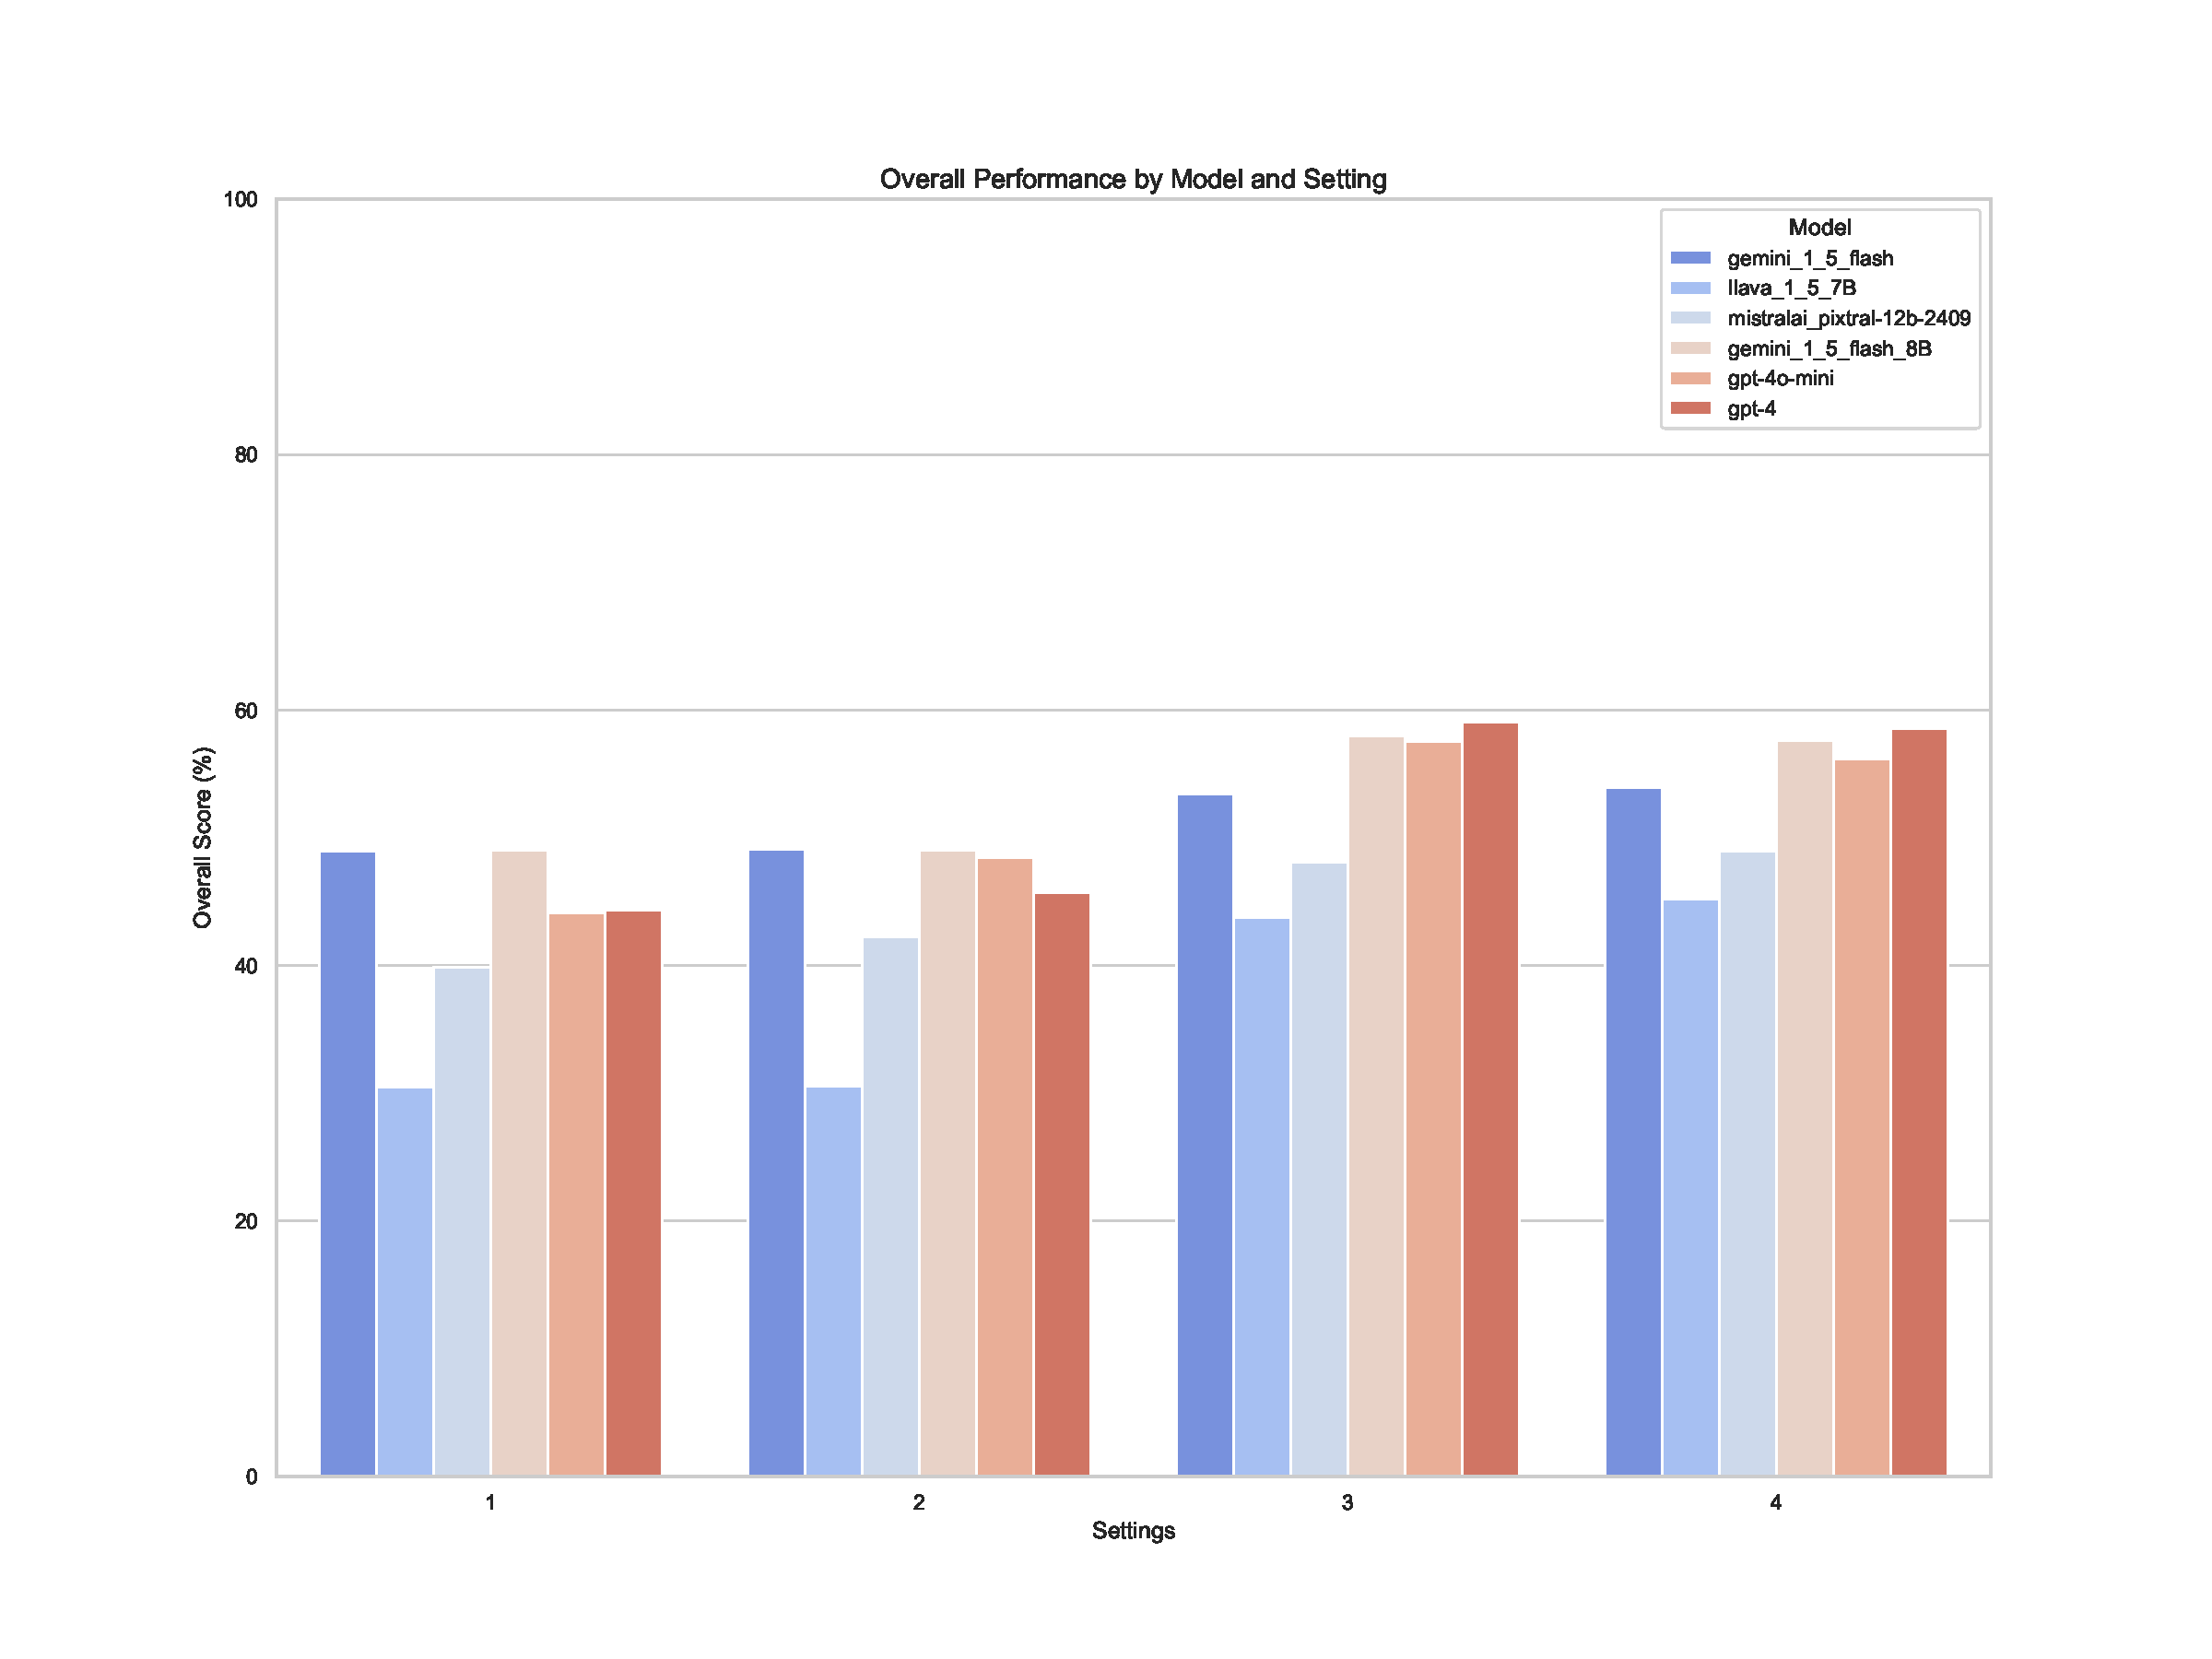
\includegraphics[width=0.8\textwidth]{images/overall_metric.pdf} 
    \caption{Overals l metrics of various LLMs.}
    \label{fig:metrics}
\end{figure}

\subsection{Summary}
The benchmarking analysis highlights the superior performance of the `Gemini` and `GPT` model families, particularly in scenarios with combined lecture and solution data. The overall score indicates that both `Gemini` and `GPT` models excel at extracting accurate answers, with `Gemini` models showing a notable advantage on datasets lacking lecture information. `GPT-4` ranked second in performance on these "pure" datasets, with only a slight difference in overall score. `Pixtral `demonstrated strong fluency despite moderate semantic alignment, while `LLaVAModel1.5-7b` showed the lowest accuracy, particularly in minimal-context settings.


\subsection{Zero-shot Benchmarking on Validation}
\subsubsection{Local Models from HuggingFace}

\paragraph{Pre-experiments} We were not successful with processing with small non-chat models. For the given text + image, the models would return short non-meaningful answers, like "Yes" to a "X or Y" question, or "no idea" to a completely defined task with all relevant context included. These were multimodal models below 1B on Huggingface, not tuned to be used in a chat scenario (and prepending a "You are a helpful assistant..." to the beginning of the prompt was not enough to fix this). 
We are not sure how to use those models for our purposes as of now. 

%Unsuccessful attempts can be mentioned in appendix I guess
%\paragraph{MiniGPT-4} This is a small multimodal model designed from ?? \cite{zhu2023minigpt}. It offers to build the model based on Llama or Vicuna. 
%\textbf{Unsuccessful experiment}: We tried to resort to an unofficial implementation: \texttt{wangrongsheng/MiniGPT-4-LLaMA-7B}. Loading the model was not successful (no preprocessor\_config.json). 
%Another issue: using BlipForConditionalGeneration and BlipProcessor: "You are using a model of type llama to instantiate a model of type blip. This is not supported for all configurations of models and can yield errors.". Model size: ~10GB. Processor: ~3.6GB. 

\paragraph{LLaVa} The exact model used is: \texttt{llava-hf/llava-1.5-7b-hf} (and there is a larger sister 13b model). It is based on LLaMA and (?) Vicuna fine-tuned on GPT-generated multimodal instruction-following data.
It expects inputs as conversation, allowing the preprocessor to convert textual input into format "USER: {request} ASSISTANT: " where the assistant has to fill in the rest. 
We encountered the following issues while applying this model version on ScienceQA data: 
\begin{itemize}
	\item although prompted like larger models, this model returned answer strings and not choice index; this may additionally raise an issue of the returned answer not being entirely part of the choice list;
	\item although prompted to generate JSON, the model would sometimes generate a different string, e.g. simply repeating part of the task. Unexpected format happened in ?? \% of all answers. We disregarded these answers, considering them all wrong, which results in a bit more pessimistic estimation of the model's performance. The metrics on the correctly formatted answers alone are also given. 
	\item the model currently does not accept inputs without an image (text-only); according to a huggingface discussion\footnote{https://huggingface.co/llava-hf/llava-1.5-7b-hf/discussions/38}, the authors claim to have accidentally removed this possibility in a recent update. We worked around this by producing placeholder empty 10x10 white images and passing them as part of the input when the image in the dataset was missing. We also appended the suffix "Ignore image" to the end of the prompt, because the model would otherwise try to hallucinate a relation between the text and the image (e.g. "Why is the sky blue" + placeholder image results in "The sky is blue on the picture because ...");
	\item the model does not really seem to support batch processing; although officially the technical possibility exists, it has been reported online \footnote{https://huggingface.co/llava-hf/llava-1.5-13b-hf/discussions/10} that the model would only take into account the first image in the batch, which makes the processing useless. We did not risk to attempt the supported or custom batching and processed the filtered validation dataset 1 datapoint by 1, which took 10+ hours on GPU for inference. 
\end{itemize}

There is another available model LLaVANext, which recently started to support batching, and should have better performance. 
%Issues: https://huggingface.co/llava-hf/llava-v1.6-mistral-7b-hf/discussions/34 

Note: I later (after running the model) understood that the original model is this one: `liuhaotian/llava-v1.5-7b`. The results may thus be different from what would be expected from the model's paper. 


%\paragraph{BLIP-2}

%\paragraph{LLaMA models} -- forbidden in EU, ignore
 
%\paragraph{Gemma2} -- Paligemma has seen ScienceQA

\paragraph{Qwen models} 
%e.g. Qwen2.5-Coder
Current experiment

\paragraph{Pixtral}

\begin{table}
\centering
\begin{tabular}{rcc}
	\toprule
	Model name & llava-1.5-7b-hf & \\
	Size & 7B & \\
	Published & 09.2023 & \\
	Type & SLM & \\
	Chat model & yes & \\
	Parent models & LLaMA, Vicuna & \\
	Data & GPT-generated multimodal instruction-following data & \\
	\bottomrule
\end{tabular}
\caption{Model Comparison: Benchmarked Models}
\end{table}

%The metrics used for evaluation at this point are: accuracy, \texttt{BLEU-1}, \texttt{BLEU-4}, \texttt{ROUGE}, similarity. 

%\section{Approximate Timeline}
%\begin{enumerate}
%	\item \textbf{Now - mid November}: 
%		\begin{itemize}
%  			\item Preliminary baseline tests: compare "pure LLM"s relying only on commonsense reasoning / only on pretraining (zero-shot, few-shot).
%			\item Stronger baseline – same LLM with better prompting techniques like CoT/Self-Ask.
%		\end{itemize}
%	\item \textbf{mid November - mid December}:
%		\begin{itemize}
 % 			\item Construct agentic / RAG pipeline with “big smart” model + additional resources.
%  			\item Optional: soft-prompting for better workflow to distill from.
%		\end{itemize}
%	\item \textbf{mid December - mid January}:
%  		\begin{itemize}
%			\item Knowledge distillation experiments.
%		\end{itemize}
%\end{enumerate}

\section{Knowledge Distillation \& Soft Prompting}
\label{knowledge-distillation}

\section{Error Analysis}
\label{error-analysis}

\section{Conclusion}
\label{Conclusion}

%\printbibliography
\bibliography{example_paper}
\bibliographystyle{icml2021}

\end{document}
